%#########################################################################
\chapter{Preliminares}
\label{cha:prem}
%#########################################################################


%*************************************************************************
\section{Motivación}
\label{sec:motiv}


La física ha evolucionado hasta un estado actual donde la mayoría de 
cálculos teóricos necesarios para realizar investigación de frontera 
requieren de una gran componente computacional. Desde la corroboración 
entre teoría y experimento, la predicción y control de los resultados de 
un experimento hecho a posteriori y la recreación de condiciones imposibles 
de lograr experimentalmente, tales como simulaciones cosmológicas del 
universo a gran escala o complejos sistemas atómicos. Estos son sólo 
algunos ejemplos representativos del papel de la computación en la física 
moderna. Debido a esto, el principal objetivo del suplemento computacional 
es la introducción temprana en los cursos de física básica de herramientas 
computacionales que serán de utilidad a los estudiantes en este curso 
específico y durante el transcurso de sus carreras científicas.


%*************************************************************************




%*************************************************************************
\section{Instalación de Paquetes}
\label{sec:install}


En la totalidad de esta guía será usado el lenguaje de programación \python
como referente para todos las prácticas y ejercicios computaciones. La 
principal motivación de esto es su facilidad de implementación en 
comparación a otros lenguajes también de amplio en ciencia. Además es un 
lenguaje interpretado, lo que permite una depuración más sencilla por 
parte del estudiante, sin necesidad de usar más complicados sistemas de 
depuración en el caso de lenguajes compilados como C o Fortran. \python es 
un lenguaje de código abierto, lo que permite la libre distribución del 
paquete y evita el pago de costosas licencias de uso, además la gran 
mayoría de paquetes que extienden enormemente la funcionalidad de \python 
son también código abierto y de libre distribución y uso.

\

A pesar de que \python es un lenguaje multiplataforma, permitiendo correr 
scripts python en Linux, Windows y Mac, acá solo se indicará el método de 
instalación para distribuciones Linux basadas en Debian.

\

La última versión de \python de la rama 2 es 2.7.4 y de la rama 3 es la 
3.3.1, debido a ligeras incompatibilidades entre ambas ramas de desarrollo, 
será utilizada la rama 2 en una de sus últimas versiones. En orden, para 
instalar \python en una versión Linux basta con descargarlo directamente 
de los repositorios oficiales\footnote{En la mayoría de distribuciones Linux
\python viene precargado por defecto.}, en el caso de una distro basada 
en Debian el gestor de paquetes es \texttt{apt-get}, y desde una terminal 
se tiene


%.........................................................................
%Install python
\begin{listing}[style=consola, numbers=none]
\$ apt-get install python2.7
\end{listing}
%.........................................................................


también puede descargarse directamente desde la página oficial del proyecto 
\url{http://python.org/}.

\

Una vez instalada la última versión de \python, es necesario instalar los
siguiente paquetes para el correcto desarrollo de las aplicaciones del 
curso:


%-------------------------------------------------------------------------
%Ipython
\subsection*{iPython}

\ipython es un shell que permite una interacción más interactiva con los
scripts de python, permitiendo el resaltado de sintaxis desde consola, 
funciones de autocompletado y depuración de código más simple. Para su 
instalación basta descargarlo de los repositorios oficiales 


%.........................................................................
%Install ipython
\begin{listing}[style=consola, numbers=none]
\$ apt-get install ipython
\end{listing}
%.........................................................................


o puede de descargarse de la página oficial \url{http://ipython.org/}. 
También puede encontrarse documentación completa y actualizada en esta 
página, se recomienda visitarla frecuentemente para tener las más recientes 
actualizaciones.


%-------------------------------------------------------------------------




%-------------------------------------------------------------------------
%NumPy
\subsection*{NumPy}

\numpy es una librería que extiende las funciones matemáticas de \python, 
permitiendo el manejo de matrices y vectores. Es esencial para la 
programación científica en \python y puede ser instalada de los repositorios


%.........................................................................
%Install NumPy
\begin{listing}[style=consola, numbers=none]
\$ apt-get install python-numpy
\end{listing}
%.........................................................................


La última versión estable es la 1.6.2. En la página oficial del proyecto 
puede encontrarse versiones actualizadas y una amplia documentación 
\url{http://www.numpy.org/}.

%-------------------------------------------------------------------------




%-------------------------------------------------------------------------
%SciPy
\subsection*{SciPy}

\scipy es una amplia biblioteca de algoritmos matemáticos para \python, 
esta incluye herramientas que van desde funciones especiales, integración,
optimización, procesamiento de señales, análisis de Fourier, etc. Al igual
que los anteriores paquetes, puede ser instalada desde los repositorios 
oficiales


%.........................................................................
%Install SciPy
\begin{listing}[style=consola, numbers=none]
\$ apt-get install python-scipy
\end{listing}
%.........................................................................


Una completa documentación del paquete puede ser encontrada en 
\url{http://docs.scipy.org/doc/scipy/reference/}. La última versión estable
es la 0.11.0 y puede ser encontrada en la página oficial del proyecto 
\url{http://www.scipy.org/}.


%-------------------------------------------------------------------------




%-------------------------------------------------------------------------
%Matplotlib
\subsection*{Matplotlib}

\matplotlib es una completa librería con rutinas para la generación de 
gráficos a partir de datos. Aunque en su estado actual está enfocada 
principalmente a gráficos 2D, permite un amplio control sobre el formato 
de las gráficas generadas, dando una amplia versatilidad a los usuarios.
Su instalación puede realizarse a partir de los repositorios oficiales


%.........................................................................
%Install Matplotlib
\begin{listing}[style=consola, numbers=none]
\$ apt-get install python-matplotlib
\end{listing}
%.........................................................................


La última versión estable es la 1.2.1. y puede encontrarse en la página 
oficial del proyecto \url{http://matplotlib.org/}. Una amplia documentación
está disponible en \url{http://matplotlib.org/1.2.0/contents.html}.


%-------------------------------------------------------------------------



%-------------------------------------------------------------------------
%Mayavi
\subsection*{MayaVi2}

\mayavi es una librería para la visualización científica en python, en 
especial para gráficos 3D, permitiendo funciones avanzadas como renderizado,
manejo de texturas, etc. Se encuentra en los repositorios oficiales 


%.........................................................................
%Install mayavi2
\begin{listing}[style=consola, numbers=none]
\$ apt-get install mayavi2
\end{listing}
%.........................................................................


La versión 2 es una versión mejorada de la original, estando más orientada
a la reutilización de código. Por defecto incluye una interfaz gráfica que
facilita su manejo. La página oficial del proyecto es 
\url{http://mayavi.sourceforge.net/}.

%-------------------------------------------------------------------------





%-------------------------------------------------------------------------
%Tkinter
\subsection*{Tkinter}

\tkinter es una librería para la gestión gráfica de aplicaciones in \python 
y viene por defecto instalada, aún así puede ser instalada de los 
repositorios oficiales


%.........................................................................
%Install Tkinter
\begin{listing}[style=consola, numbers=none]
\$ apt-get install python-tk
\end{listing}
%.........................................................................


La página oficial del proyecto es \url{http://wiki.python.org/moin/TkInter}.
Para el desarrollo de entornos gráficos existen otras llamativas
alternativas como PyGTK o PyQt, pero debido a la facilidad de uso y a ser
la librería estándar soportada, \tkinter será usada en este curso.


%-------------------------------------------------------------------------


%*************************************************************************





%*************************************************************************
\section{Ejemplo de Uso}
\label{sec:usage}


En esta sección se ilustra un ejemplo sencillo que permite al estudiante 
identificar la manera estándar de ejecutar códigos en \python, además probar 
los paquetes instalados.

\

El código de ejemplo permite graficar dos funciones diferentes en una misma
ventana y además un conjunto de datos aleatorios generados en el eje Y.


%ccccccccccccccccccccccccccccccccccccccccccccccccccccccccccccccccccccccccc
%USAGE_01
\begin{listing}[style=python]
#!/usr/bin/env python
#==========================================================
# EJEMPLO DE USO
# Grafica de funciones y datos aleatorios
#==========================================================
import numpy as np
import scipy as sp
import matplotlib.pylab as plt

#Funcion 1
def Funcion1(x):
    f1 = np.sin(x)/( np.sqrt(1 + x**2) )
    return f1
    
#Funcion 2
def Funcion2(x):
    f2 = 1/(1+x)
    return f2
    
#Valores de x para evaluar
X = np.linspace( 0, 10, 100 )
#Evaluacion de funcion 1
F1 = Funcion1(X)
#Evaluacion de funcion 2
F2 = Funcion2(X)

#Grafica funcion 1
plt.plot( X, F1, label='Funcion 1' )
#Grafica funcion 2
plt.plot( X, F2, label='Funcion 2' )

#Datos aleatorios eje Y
Yrand = sp.random.rand( 100 )
#Grafica datos aleatorios
plt.plot( X, Yrand, 'o', label='Datos' )

plt.legend()
plt.show()
\end{listing}
%ccccccccccccccccccccccccccccccccccccccccccccccccccccccccccccccccccccccccc


El resultado obtenido es la siguiente gráfica

%.........................................................................
%Simple Pendulum Exact solution
\begin{figure}[htbp]
	\centering
	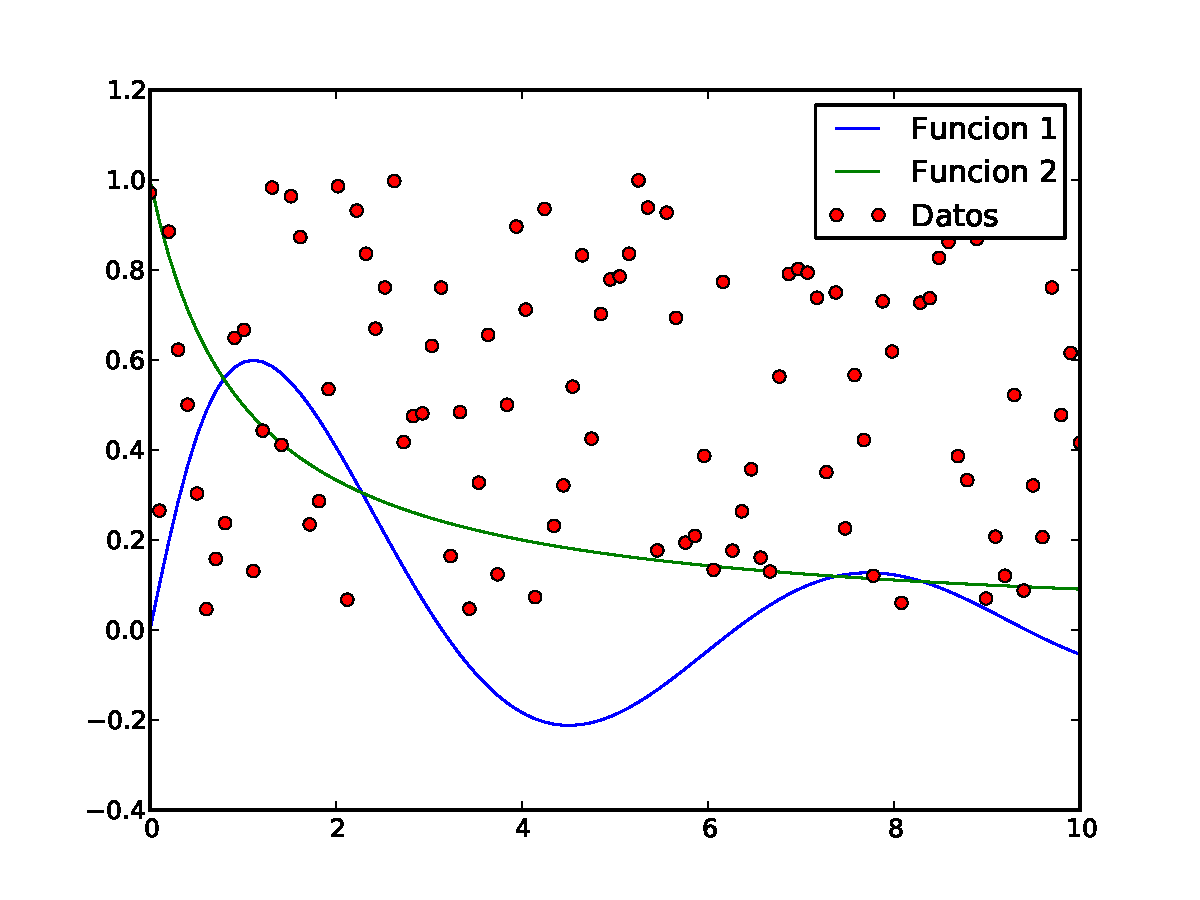
\includegraphics[width=0.7\textwidth]
	{./pictures/usage_01.pdf}

	\caption{\small{Resultado del ejemplo anterior, gráfica de dos funciones
	y datos aleatorios.}}
	
	\label{fig:small_pedulum}
\end{figure}
%.........................................................................


Para obtener el anterior script, el estudiante puede transcribirlo 
directamente de esta guía o puede descargarlo del repositorio oficial del 
curso\footnote{Repositorio oficial en 
\url{https://github.com/sbustamante/Computacional-Campos}} en el link
\url{https://github.com/sbustamante/Computacional-Campos/raw/master/codigos/usage\_01.py}.
Una vez obtenido el archivo \texttt{usage\_01.py}, abrir una terminal en la 
carpeta donde se ha guardado y escribir \texttt{ipython} para abrir el 
intérprete de \python


%.........................................................................
%Opening iPython
\begin{listing}[style=consola, numbers=none]
\$ ipython
\end{listing}
%.........................................................................


Se debe obtener algo como


%.........................................................................
%iPython
\begin{listing}[style=consola, numbers=none]
\$ ipython
Python 2.6.5 (r265:79063, Apr 16 2010, 13:57:41) 
Type "copyright", "credits" or "license" for more information.

IPython 0.10 -- An enhanced Interactive Python.
?         -> Introduction and overview of IPython's features.
%quickref -> Quick reference.
help      -> Python's own help system.
object?   -> Details about 'object'. ?object also works, ?? prints more.

In [1]: 
\end{listing}
%.........................................................................


Finalmente para ejecutar el script, usar el comando \texttt{run} seguido
del nombre del código en el intérprete de código \python


%.........................................................................
%Runing a script
\begin{listing}[style=consola, numbers=none]
In [1]: run usage_01.py
\end{listing}
%.........................................................................

%*************************************************************************




%*************************************************************************
\section{Consejos de Programación}
\label{sec:advice}


En esta sección se dan algunos consejos útiles a la hora de programar. 
Estas buenas prácticas ayudan al programador a ser estructurado y tener 
un método coherente de desarrollar códigos.


%.........................................................................
\begin{itemize}
\item Asignar nombres a los archivos que sean coherentes con lo que realizan. 
Por ejemplo si está realizando una rutina que integra la trayectoria de una 
partícula en un campo eléctrico $\bds E$, un nombre adecuado para el código
puede ser \texttt{trayectory\_electric\_field.py}. Evite usar nombres poco
intuitivos y que tengan caracteres extraños, inclusive caracteres tildados 
como \texttt{í}, \texttt{ó}, \texttt{ñ}, etc. También evite el uso de 
espacios, si desea separar palabras, use el caracter \texttt{\_}.

\item Una práctica casi obligatoria que debe realizar cualquier programador 
serio, consiste en comentar su código exhaustivamente. Los lenguajes de 
programación fueron inventados para facilitar la interacción entre el 
humano y la computadores, los compiladores e intérpretes de códigos 
\textit{traducen} este lenguaje a lenguaje binario de máquina. Es por esta 
razón que cuando se crea un código, se debe pensar en que este sea 
comprensible, siempre recuerde que la máquina solo requiere código binario.

\

Comente todo lo que usted crea conveniente. Es muy común que por minimizar 
líneas de código o simplemente por pensar que no es necesario, muchos 
programadores dejan de comentar su código y semanas más tarde retoman y no 
entienden que han hecho. La programación en equipo es cada vez más común 
en ciencia, existiendo grandes proyectos donde una comunidad activa está 
contribuyendo, comentar el código es indispensable para este tipo de 
actividades.

\item Use el inglés siempre que pueda, para asignar nombres a sus archivos, 
para comentar su código, y para datos impresos en pantalla y en archivos de 
datos. Tenga en cuenta que en disciplinas científicas cualquier labor que 
sea realizada en inglés tendrá un potencial de impacto mayor que otro si se 
hace en otro idioma. Su código puede ser útil después a otras personas y 
esto puede ayudar a que usted sea reconocido en círculos académicos.

\item Comparta su código, para esto puede usar páginas diseñadas para esto
tales como \url{github.com} o \url{sourceforge.net}. Estas páginas además
de permitir compartir su código a terceras personas, tiene potentes 
herramientas de control de versiones (git, svn, etc.) las cuales le ayudan 
a manejar su código de forma más estructurada, permitiendo el control de 
las diferentes versiones de un código o un paquete completo y el desarrollo
entre varias personas.

\item Use software open source, este tipo de software es de libre 
distribución y uso. Cuando se usan herramientas que necesitan licencia se
está sujeto al pago de ingentes cantidades de dinero por funcionalidades
que se pueden encontrar de forma gratuita. Este tipo de herramientas pagas
limitan aspectos como el poder compartir códigos y resultados, por ejemplo 
si usted no tiene su licencia al día puede tener problemas a la hora de 
reportar en un artículo de investigación sus resultados y gráficas obtenidos 
con estos paquetes.

\end{itemize}
%.........................................................................


%*************************************************************************